\section{Auswertung}
\label{sec:Auswertung}

\subsection{Überprüfen der Stabilitätsbesingung}
\label{sec:Überprüfen der Stabilitätsbesingung}

Für die Stabilitätsbedingung gilt Gleichung 1EINFÜGEN, daraus ergibt sich für einen Resonator bestehend aus einem planen und einem konkaven Spiegel, 
die Bedingung,

\begin{equation}
\label{equ:}
  0 \leq L \leq r_{konkav}
\end{equation}
und für zwei konkave Spiegel,

\begin{equation}
\label{equ:}
  0 \leq L \leq 2 \cdot r_{konkav}.
\end{equation}
Für den ersten verwendeten Resonator mit einem planen Spiegel und einem konkaven Spiegel mit Krümmungsradius $r_1 = 140 \: cm$ gilt somit der 
theoretische maximale Resonatorabstand von $L_{max} = 140 \: cm$.
Bei dem zweiten Resonator mit zwei konkaven Spiegeln mit $g_2 = g_3 = 140 \: cm$ beträgt der Theoriewert $L_{max} = 280 \: cm$.
Bei dem ersten Resonator konnte bei den Meesungen ein Laser bis zu einer Resonatorlänge von $L_{real} = 144,5 \: cm$ erzeugt werden,
also größer als der theoretisch mögliche Wert.
Beim zweiten Resonator bis $L_{real} = 217,5 \: cm$, da dort allerdings das Ende der Optischen Schiene war, konnte die Stabilitätsbedingung nicht weiter getestet werden.

In Tabelle \ref{tab:1} sind die eingestellten Resonatorlängen mit entsprechenden Intensitäten angegeben.


\begin{table}[H]
  \centering
  \footnotesize
  \caption{Intensitätsmesswerte $I(L)$ der beiden Resonatorkonfigurationen.}
  \label{tab:1}
  \begin{tabular}{r r | r r}
  \toprule
  $L_{pk} \;/\; \si{\centi\meter}$ & $I_{pk} \;/\; \si{\milli\watt}$ & $L_{kk} \;/\; \si{\centi\meter}$ & $I_{kk} \;/\; \si{\milli\watt}$ \\
  \midrule
  112   & 1,6 & 86,1 & 3,5 \\
  125   & 1,7 & 94,8 & 3,8 \\
  144,5 & 0,8 & 119 & 2,6 \\
  /     & /   & 148,6 & 2,5 \\
  /     & /   & 156,1 & 4,1 \\  
  /     & /   & 189,2 & 5,7 \\
  /     & /   & 217,5 & 4,0 \\
  \bottomrule
  \end{tabular}
\end{table}


\subsection{Beobachtung von TEM-Moden}
\label{sec:Beobachtung von TEM-Moden}
Als TEM-Moden werden die Moden bezeichnet, welche in der Ebene senkrecht zur Ausbreitungsrichtung des Lasers, 
die Intensitätsverteilung bestimmen. Also die transversalen Moden des Lasers.

\subsubsection{Beobachung der TEM_{00}-Mode}
\label{sec:Beobachung der 00-Mode}
Die theoretische Intensitätsverteilung der $\text{TEM_{00}-Mode}$ entspricht einer Gaußverteilung. Daher werden die Messdaten aus Tabelle \ref{tab:TEM00} im Graphen \ref{fig:TEM00} geplottet,
so wie eine entsprechend der Daten gefittete Gaußfunktion. Die Form der Gußfunktion sieht wie folgt aus:

\begin{equation}
\label{equ:}
  I_{00}(r) = I_0 \cdot exp \left(- \frac{(r - r_0)^2}{2 \omega^2}\right) + I_{off}
\end{equation}
Mit dem Offser $I_{off} = 0,2 \: \si{\micro\watt}$ und den Parametern:
$I_0 = EINFÜGEN$
$r_0 = EINFÜGEN$
$\omega = EINFÜGEN$


\begin{table}[H]
  \centering
  \footnotesize
  \caption{Messwerte der Intensität $I(r)$ der TEM$_{00}$-Mode.}
  \label{tab:TEM00}
  \begin{tabular}{r r}
  \toprule
  $r \;/\; \si{\milli\meter}$ & $I \;/\; \si{\micro\watt}$ \\
  \midrule
-11 & -0.06   \\
-10 & 0.12    \\
-9  & 0.47    \\
-8  &  0.84   \\
-7  &  1.7    \\
-6  &  2.9    \\
-5  &  4.6    \\
-4  &  7    \\
-3  &  10   \\
-2  &  14   \\
-1  &  19   \\
0   &  26   \\
1   &  29   \\
2   &  30   \\
3   &  32   \\
4   &  32   \\
5   &  29   \\
6   &  25   \\
7   &  20   \\
8   &  16   \\
9   &  11   \\
10  &  7    \\
11  &  4,4    \\
12  &  2,6    \\
13  &  1,4    \\
14  &  0,66   \\
15  &  0,23   \\
15  &  -0,01    \\
16  &  -0,13    \\
  \bottomrule
  \end{tabular}
\end{table}

\begin{figure}[H]
  \centering
  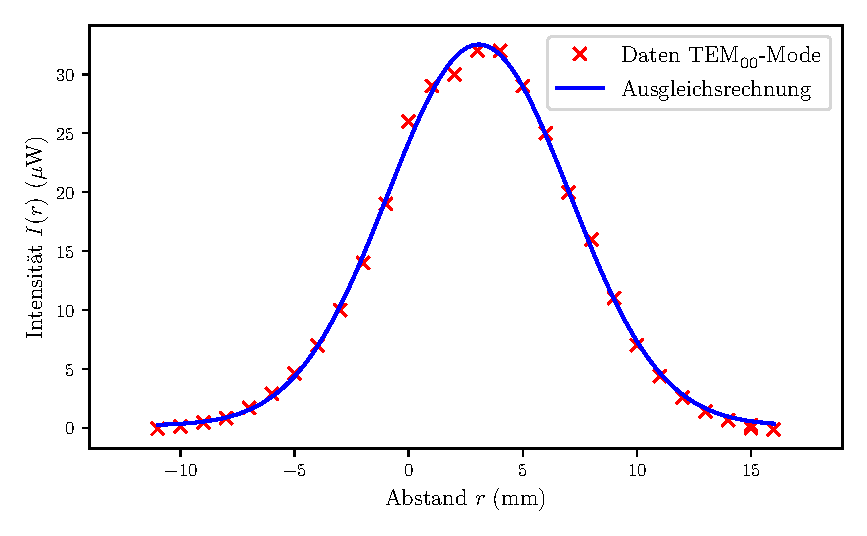
\includegraphics[scale=0.65]{content/TEM00.pdf}
  \vspace{-10pt}
  \caption{Intensitätsverteilung $I(r)$ der TEM$_{00}$-Mode.}
  \label{fig:TEM00}
\end{figure}


\subsubsection{Beobachtung der TEM$_{10}$-Mode}
\label{sec:Beobachtung der EINFÜGEN-Mode}
Um die 10-Mode messen zu können wird ein dünner Draht in den Resonator gebracht.
Dieser Draht verursacht eine Störung der Moden und unterdrückt diese somit. Befindet sich der Draht genau an der Stelle eines Maximums der Grundmode $\text{TEM_{00}}$, so wird diese maximal gestört.
Gleichzeitig wird die 10-Mode minimal gestört, da sich an der stelle des Drahtes gerade ein Minimum dieser Mode befindet. Dies führt dazu, dass die 10-Mode beobachtet werden kann.
Die Messwerte der Intensitätsverteilung der TEM$_{10}$-Mode sind in Tabelle \ref{tab:TEM10} aufgelistet. Diese sind nicht einfach Gaußförmig und werden entsprechend der Funktion

\begin{equation}
  I_01(r) = I_0 \cdot \frac{8 (r - r_0)^2}{\omega^2} \cdot \left( - \frac{2 (r - r_0)^2}{\omega^2}\right) + I_{off},
\end{equation}
gefittet. Die Gefittete Funktion und die Messdaten sind in Graph \ref{fig:TEM01} abggebildet.


\begin{table}[H]
  \centering
  \footnotesize
  \caption{Messwerte der Intensität $I(r)$ der TEM$_{10}$-Mode abhängig vom Modenmittenabstand $r$.}
  \label{tab:TEM10}
  \begin{tabular}{r r}
  \toprule
  $r \;/\; \si{\milli\meter}$ & $I \;/\; \si{\micro\watt}$ \\
  \midrule
    -11 & -0,02 \\
    -10 & 0,11  \\
    -9  & 0,33  \\
    -8  & 0,57  \\
    -7  & 0,9   \\
    -6  & 1,4   \\
    -5  & 1,9   \\
    -4  & 2,3   \\
    -3  & 2,8   \\
    -2  & 2,8   \\
    -1  & 2,5   \\
    0   & 1,4   \\
    1   & 0,8   \\
    2   & 0,14  \\
    3   & -0,17 \\
    4   & 0,07  \\
    5   & 0,68  \\
    6   & 1,7   \\
    7   & 2,2   \\
    8   & 2,3   \\
    9   & 2,4   \\
    10  & 2,2   \\
    11  & 1,7   \\
    12  & 1,3   \\
    13  & 0,99  \\
    14  & 0,58  \\
    15  & 0,26  \\
    16  & 0,03  \\
    17  & -0,1  \\
  \bottomrule
  \end{tabular}
\end{table}


\begin{figure}[H]
  \centering
  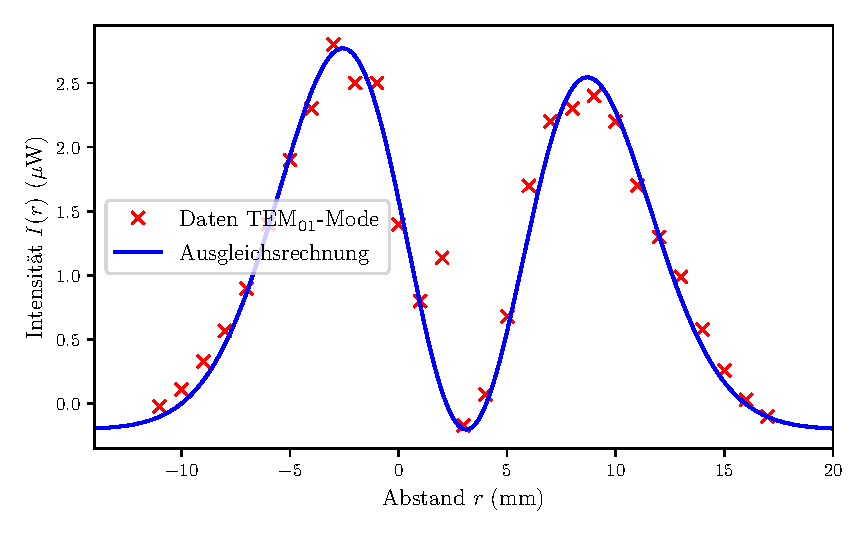
\includegraphics[scale=0.65]{content/TEM01.pdf}
  \vspace{-10pt}
  \caption{Intensitätsverteilung $I(r)$ der TEM$_{01}$-Mode.}
  \label{fig:TEM01}
\end{figure}


\subsection{Bestimmung der Polarisation}
\label{sec:estimmung der Polarisation}
Die Daten der Polarisationsmessung, also die gemessenen Intensitäten in abhängigkeit vom Polarisationswinkel, sind in Tabelle \ref{tab:pol} aufgelistet.
Die Intensitätsverteilung sollte einer Funktion der Form,

\begin{equation}
\label{equ:}
  I(\phi) = I_0 \cdot cos^2((\phi + \phi_0) \cdot \frac{2 \pi}{360^{\circ}}),
\end{equation}
gleichen.
Daher wird eine entsprechende Funktion entsprechend der Messwerte gefittet und in Graph \ref{fig:pol}, zusammen mit den Messwerten eingetragen.
Die Parameter die sich für die Funktion ergeben sind:
$I_0 = EINFÜGEN$
$\phi_0 = EINFÜGEN$


\begin{table}[H]
  \centering
  \footnotesize
  \caption{Messwerte der Intensität $I(\phi)$ abhängig vom Polarisationswinkel $\phi$.}
  \label{tab:pol}
  \begin{tabular}{r r}
  \toprule
  $\phi \;/\; \si{\degree}$ & $I \;/\; \si{\micro\watt}$ \\
  \midrule
    0   & 0,82 \\
    10  & 26   \\ 
    20  & 115  \\
    30  & 230  \\
    40  & 270  \\
    50  & 450  \\
    60  & 650  \\
    70  & 780  \\
    80  & 840  \\
    90  & 860  \\
    100 & 830  \\
    110 & 770  \\
    120 & 630  \\
    130 & 490  \\
    140 & 340  \\
    150 & 200  \\
    160 & 90   \\
    170 & 22   \\
    180 & 0,9  \\
    190 & 32   \\
  \bottomrule
  \end{tabular}
\end{table}


\begin{figure}[H]
  \centering
  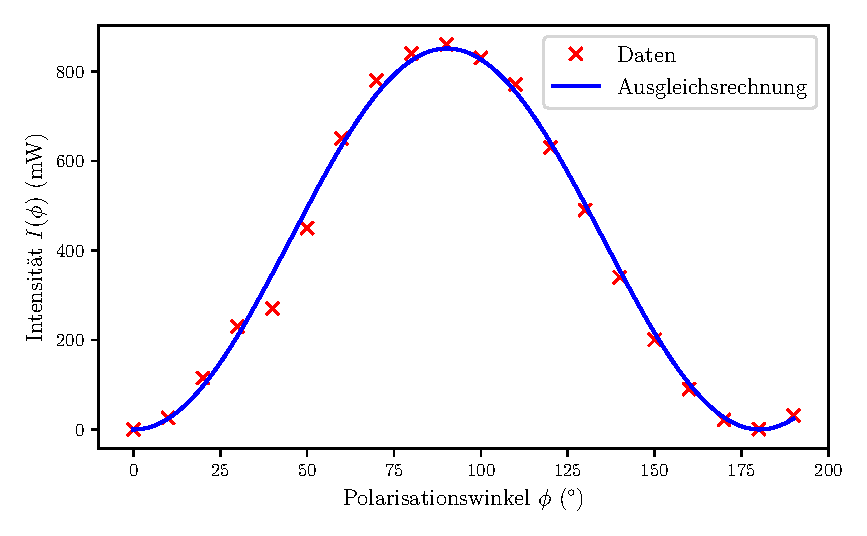
\includegraphics[scale=0.65]{content/pol.pdf}
  \vspace{-10pt}
  \caption{Intensitätsverteilung $I(\phi)$ in Abhängigkeit vom Polarisationswinkel $\phi$.}
  \label{fig:pol}
\end{figure}



\subsection{Multimodenbetrieb}
\label{sec:Multimodenbetrieb}
Die Frequenz der verschiedenen longitudinalen Moden, abhängig von der Resonatorlänge wird beschrieben durch,

\begin{equation}
\label{equ:}
  f = \frac{n \cdot c}{2L},
\end{equation}
 woraus sich für die Modendifferenz,

 \begin{equation}
\label{equ:Modendifferenz}
  \Delta f = \frac{c}{2L},
\end{equation}
ergibt. Hierbei ist $L$ die Resonatorlänge und $c$ die Lichtgeschwindigkeit.
Die für verschiedene Resonatorlängen aufenommenen Messwerte sind in Tabelle \ref{tab:lon} aufgelistet. 
Die sich daraus ergebenen Frequenzdifferenzen sind zusammen mit den durch Gleichung \eqref{equ:Modendifferenz} berechneten Werten, in Tabelle \ref{tab:lon2} aufgelistet.
Die mit der Modendifferenz zu vergleichende Verbreiterung des Neonübergangs, durch den Dopplereffekt, wird durch 

\begin{equation}
  \partial f_D = \frac{f_0}{c} \sqrt{\frac{8 k_B T ln(2)}{m}},
\end{equation}
bei einer Raumtemperatur von $T=300 \: K$, zu 
$\partial f_D = 1308,21$ \: MHz
berechnet. 


\begin{table}[H]
  \centering
  \footnotesize
  \caption{Messwerte der Frequenz der fouriertransformierten Peaks der longitudinalen Moden.}
  \label{tab:lon}
  \begin{tabular}{r r r r r}
  \toprule
      & d = 86,1 \: cm & d = 94,8 \: cm & d = 119 \: cm & d = 156,1 \: cm  \\
    n & f / MHz & f / MHz  & f / MHz & f / MHz \\
  \midrule
    1 & 173 & 158 & 128 & 101 \\
    2 & 349 & 315 & 255 & 191 \\
    3 & 521 & 476 & 379 & 289 \\
    4 & 694 & 634 & 506 & 390 \\
    5 & 870 & 791 & 634 & 484 \\
    6 & /   & 949 & 758 & 578 \\
    7 & /   & /   & 885 & 675 \\
    8 & /   & /   & /   & 769 \\
  \bottomrule
  \end{tabular}
\end{table}


\begin{table}[H]
  \centering
  \footnotesize
  \caption{Frequenzdifferenz Messwerte und Theoriewerte.}
  \label{tab:lon2}
  \begin{tabular}{r r r}
  \toprule
    L / cm & $\Delta$ f$_{mes}$ / MHz & $\Delta$ f$_{the}$ / MHz \\
      86,1 & 174,25 & 174,10 \\
      94,8 & 158,2  & 158,12 \\
      119  & 126,17 & 125,96 \\
      156,1& 95,42  & 96,03  \\
  \bottomrule
  \end{tabular}
\end{table}



\subsection{Bestimmung der Wellenlänge}
\label{sec:Bestimmung der Wellenlänge}
Die Wellenlänge des Lasers kann durch Beugungsmuster an einem Spalt bzw. Gitter bestimmt werden. 
Dazu werden die Abstände $d_n$ der Beugungsmaxima zur optischen Achse gemessen.
Diese Abstände sind in Tabelle \ref{fig:wel} aufgelistet.

Aus diesen Abständen und dem Abstand zwischen Gitter und Schirm $l$, kann durch

\begin{equation}
  \lambda = \frac{sin \left(tan \left(\frac{d_n}{l}\right)\right)}{n \cdot g}
\end{equation}
die Wellenlänge bestimmt werden. Dabei ist $g$ der Gitterabstand. 

Die so berechneten Wellenlängen ergeben für das erste Gitter einen Mittelwert von 
$\lambda = EINFÜGEN$ 
und für das zweite Gitter
$\lambda = EINFÜGEN$.
Der gesamte Mitterwert für die Wellenlänge des Lasers ist somit
$\lambda = EINFÜGEN$.


\begin{table}[H]
  \centering
  \footnotesize
  \caption{Messwerte für die Wellenlängenbestimmung}
  \label{tab:wel}
  \begin{tabular}{r r r}
  \toprule
    n & $d_{n,g1}$ / cm & $d_{n,g2}$ / cm \\
  \midrule
    -8 & 23,7 & 29,5 \\
    -7 & 20,0 & 25,9 \\
    -6 & 16,8 & 21,3 \\
    -5 & 13,5 & 17,4 \\
    -4 & 10,9 & 13,3 \\
    -3 & 8,2  & 9,9 \\
    -2 & 5,4  & 6,5 \\
    -1 & 2,7  & 3,5 \\
    0  & 0    & 0   \\
    1  & 2,7  & 3,2 \\
    2  & 5,3  & 6,3 \\
    3  & 7,9  & 9,4 \\
    4  & 10,7 & 12,5 \\
    5  & 13,4 & 16,0 \\
    6  & 16,2 & 19,7 \\
    7  & 19,1 & 23,3 \\ 
    8  & 22,3 & 27,5 \\
    9  & 25,8 & 33,3 \\
    10 & 29,5 & /    \\
    11 & 33,5 & /    \\
    12 & 38,0 & /    \\
  \bottomrule
  \end{tabular}
\end{table}
